\documentclass[10pt,twocolumn,letterpaper]{article}

\usepackage{cvpr}
\usepackage{times}
\usepackage{epsfig}
\usepackage{graphicx}
\usepackage{amsmath}
\usepackage{amssymb}
\usepackage{caption}
\usepackage{verbatim}
\usepackage{subcaption}
\usepackage{algorithm2e}
\usepackage{rotating}

\usepackage[space]{grffile}
\usepackage[font=small,skip=0pt]{caption}
%\DeclareMathOperator{\Tr}{Tr}
% Include other packages here, before hyperref.

% If you comment hyperref and then uncomment it, you should delete
% egpaper.aux before re-running latex.  (Or just hit 'q' on the first latex
% run, let it finish, and you should be clear).
\usepackage[breaklinks=true,bookmarks=false]{hyperref}
\graphicspath{ {figures/} }
% \cvprfinalcopy % *** Uncomment this line for the final submission

\def\cvprPaperID{2349} % *** Enter the CVPR Paper ID here
\def\httilde{\mbox{\tt\raisebox{-.5ex}{\symbol{126}}}}

% custom commands
\newcommand{\scream}[1]{{\color{red} \bf *** #1 ***}}

% Pages are numbered in submission mode, and unnumbered in camera-ready
%\ifcvprfinal\pagestyle{empty}\fi
\setcounter{page}{1}
\begin{document}

%%%%%%%%% TITLE
\title{Supplementary Material for the Paper ``Enriching Object Detection with\\2D-3D Registration and Continuous Viewpoint Estimation''}
%\title{Enrich Object Detection : 2D-3D registration and continuous viewpoint estimation}

% \author{First Author\\
% Institution1\\
% Institution1 address\\
% {\tt\small firstauthor@i1.org}
% % For a paper whose authors are all at the same institution,
% % omit the following lines up until the closing ``}''.
% % Additional authors and addresses can be added with ``\and'',
% % just like the second author.
% % To save space, use either the email address or home page, not both
% \and
% Second Author\\
% Institution2\\
% First line of institution2 address\\
% {\tt\small secondauthor@i2.org}
% }

\maketitle
%\thispagestyle{empty}

%%%%%%%%% BODY TEXT
In the following, we present additional quantitative and qualitative
results that accompany the experiments described in Sect.~6 of the
main paper, ``Enriching Object Detection with 2D-3D Registration and
Continuous Viewpoint Estimation''.
% In Sect.~\ref{sec:3dobject}, we present detection result on qualitative results.

\section{2D-3D Matching as an Object Detector}
\label{sect:3dobject}
It this section, we provide qualitative examples and plots for the experiment
``2D-3D Matching as an Object Detector'' (Sect.~6.2 in the main
paper).

To recapitulate, we run our ensemble
of NZ-WHO templates on the 3D Object Classes
dataset~\cite{savarese07}, without the fine-tuning
stage. Fig.~\ref{fig:3dobject_ap} gives the corresponding detection
average precision, average viewpoint precision, viewpoint confusion
matrix and mean precision in pose estimation results. Specifically, we
followed the detection and viewpoint estimation criteria
of~\cite{Xiang12} where a detection is correct iff
intersection over union is at least $0.5$ and viewpoint estimation is
correct iff detection is correct \emph{and} azimuth of the viewpoint
prediction falls into the correct viewpoint bin.
%
\begin{figure}[h]
  \centering
  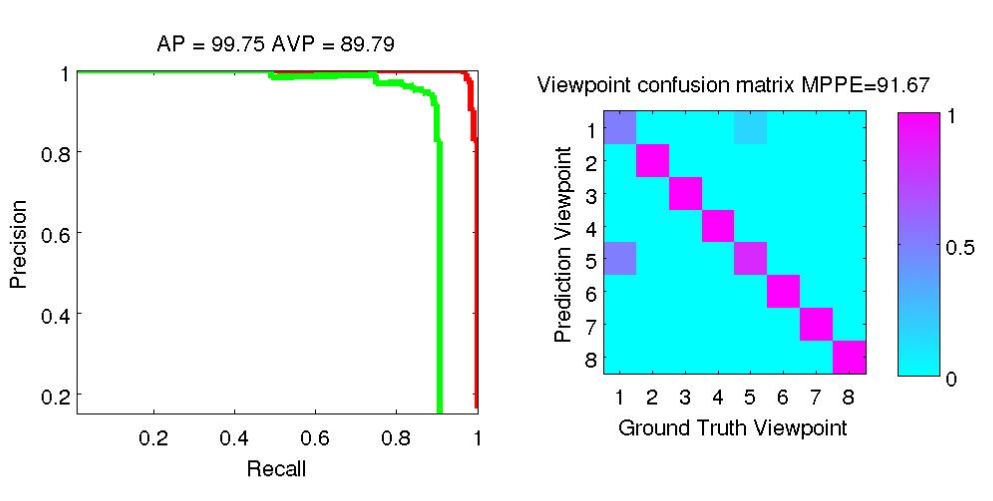
\includegraphics[width=0.99\linewidth]{supp/car_ap_3dobject_tight.png}\\
  \vspace{-5pt}
    (a) Car\\
  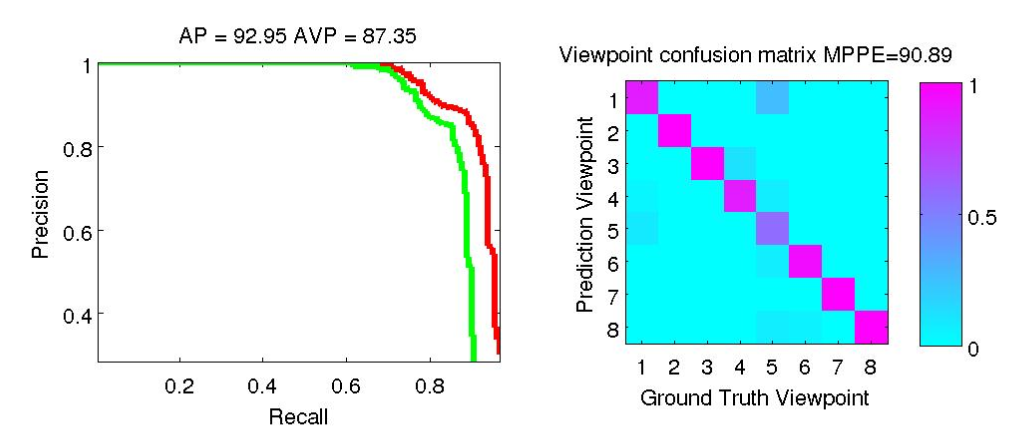
\includegraphics[width=0.99\linewidth]{supp/bicycle_ap_3dobject_tight.png}\\
  \vspace{-5pt}
    (b) Bicycle\\
  \caption{Detection and pose estimation on 3D Object
    Classes~\cite{savarese07} car (a) and bicycle (b).
    Average Precision (red) and Average Viewpoint Precision (green)
    are given in the left plot and viewpoint confusion table and MPPE
    are given in the right plot. The viewpoint index 1 is front, 2 is
    front-right, \dots, 8 is front-left.}
  \label{fig:3dobject_ap}
\end{figure}

Fig.~\ref{fig:3dobject_car_good} shows successful detection and
viewpoint estimation results for car,
Fig.~\ref{fig:3dobject_bicycle_good} for
bicycle. Fig.~\ref{fig:3dobject_car_bad} and
Fig.~\ref{fig:3dobject_bicycle_bad} show failure cases, which are
mostly due to confused front and back views for cars, and slanted
bicycle poses.


\begin{figure*}[h]
\setlength\tabcolsep{1pt}
\centering
\begin{tabular}{|c|c|}
  \hline
  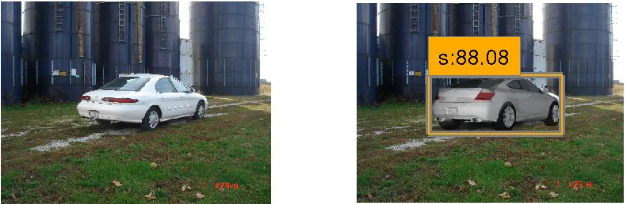
\includegraphics[width=0.40\linewidth]{supp/car32.png} &
  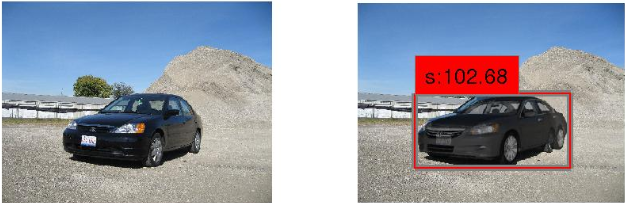
\includegraphics[width=0.40\linewidth]{supp/car26.png} \\
  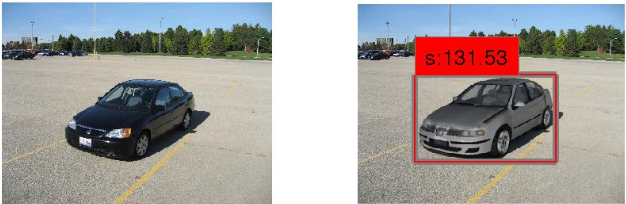
\includegraphics[width=0.40\linewidth]{supp/car29.png} & 
  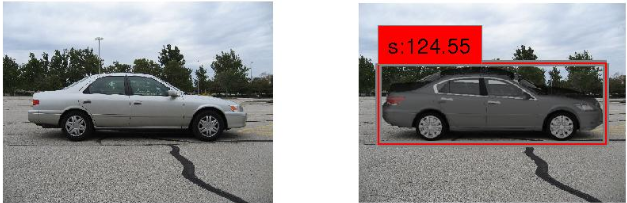
\includegraphics[width=0.40\linewidth]{supp/car10.png} \\
  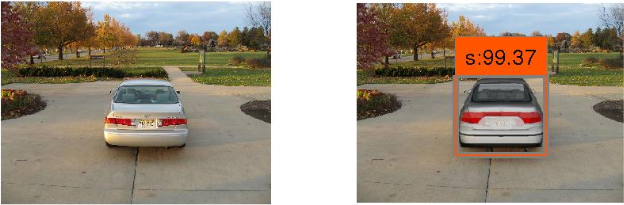
\includegraphics[width=0.40\linewidth]{supp/car1.png} &
  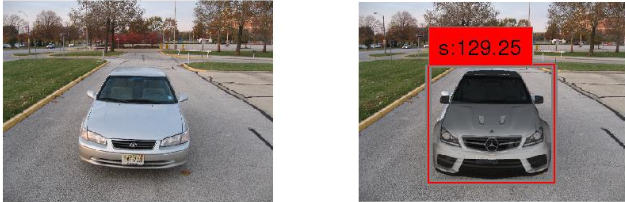
\includegraphics[width=0.40\linewidth]{supp/car8.png} \\
  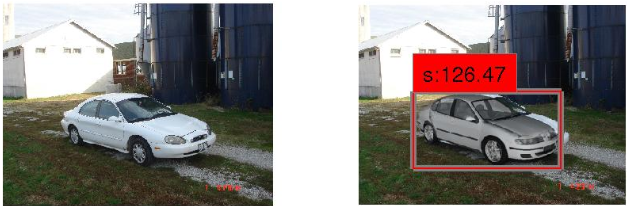
\includegraphics[width=0.40\linewidth]{supp/car20.png} & 
  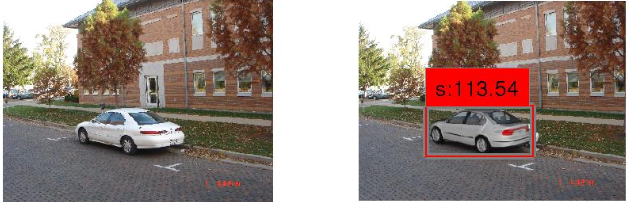
\includegraphics[width=0.40\linewidth]{supp/car31.png} \\
  \hline
  \end{tabular}
\caption{Successful detection results on 3D Object
  Classes~\cite{savarese07} cars. Original image (left) and overlaid
  detection result (right).}% with a bounding box and corresponding
                            % confidence score (right).}
  \label{fig:3dobject_car_good}
\end{figure*}

\begin{figure*}[h]
\setlength\tabcolsep{1pt}
\centering
\begin{tabular}{|c|c|}
  \hline
  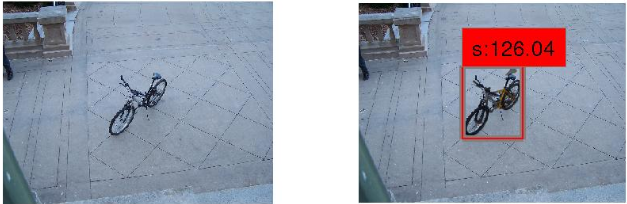
\includegraphics[width=0.40\linewidth]{supp/bicycle17.png} &
  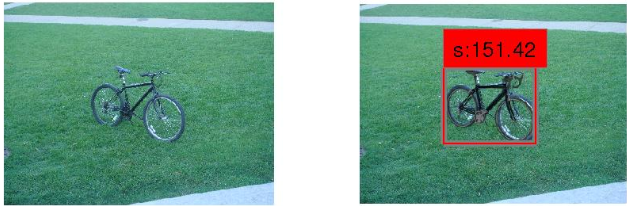
\includegraphics[width=0.40\linewidth]{supp/bicycle18.png} \\
  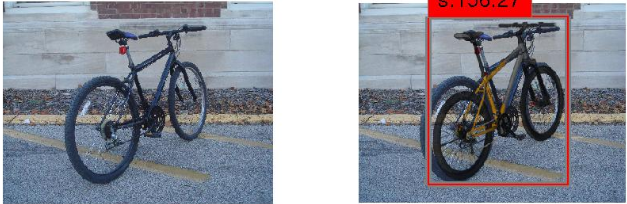
\includegraphics[width=0.40\linewidth]{supp/bicycle13.png} &
  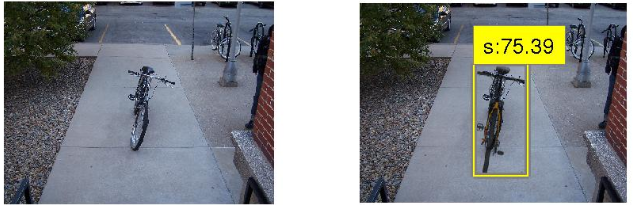
\includegraphics[width=0.40\linewidth]{supp/bicycle9.png} \\
  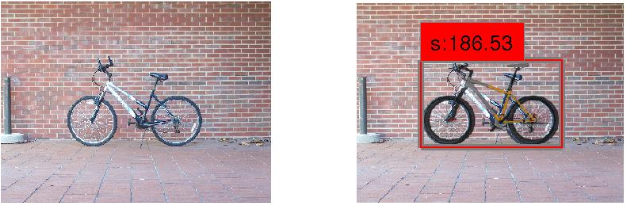
\includegraphics[width=0.40\linewidth]{supp/bicycle16.png} &
  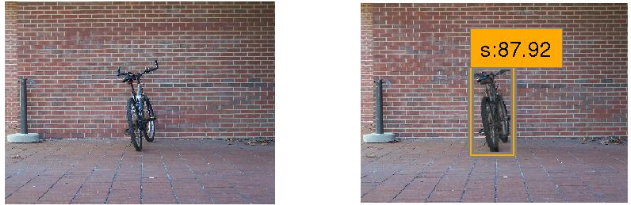
\includegraphics[width=0.40\linewidth]{supp/bicycle12.png} \\
  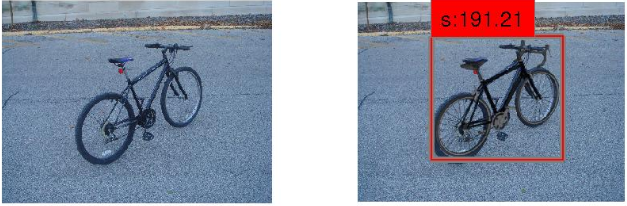
\includegraphics[width=0.40\linewidth]{supp/bicycle15.png} &
  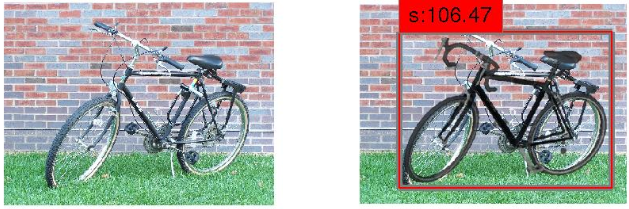
\includegraphics[width=0.40\linewidth]{supp/bicycle10.png} \\
  \hline
  \end{tabular}
\caption{Successful detection results on 3D Object
  Classes~\cite{savarese07} bicycles. Original image (left) and
  overlaid detection result (right).}
  \label{fig:3dobject_bicycle_good}
\end{figure*}

\begin{figure*}[h]
\setlength\tabcolsep{1pt}
\centering
\begin{tabular}{|c|c|}
  \hline
  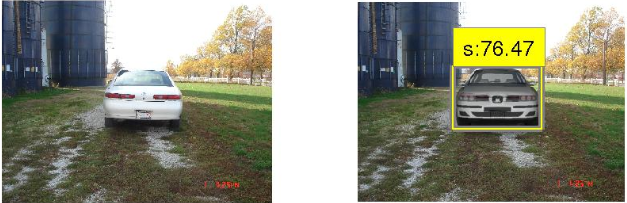
\includegraphics[width=0.40\linewidth]{supp/car13.png} &
  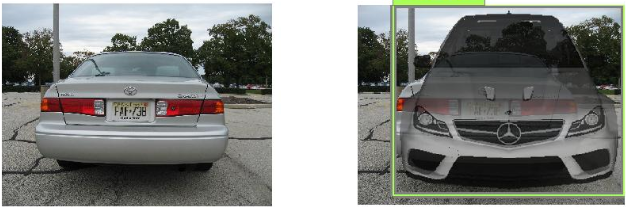
\includegraphics[width=0.40\linewidth]{supp/car30.png} \\ 
  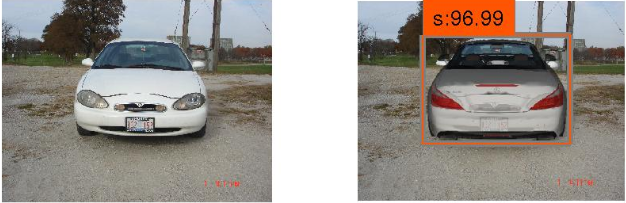
\includegraphics[width=0.40\linewidth]{supp/car18.png} &
  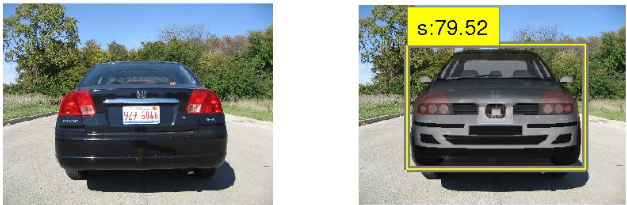
\includegraphics[width=0.40\linewidth]{supp/car25.png} \\
  \hline
  \end{tabular}
\caption{Failed detection or pose estimation on 3D Object
  Classes~\cite{savarese07} cars. Original image (left) and overlaid
  detection result (right).}
  \label{fig:3dobject_car_bad}
\end{figure*}

\begin{figure*}[h]
\setlength\tabcolsep{1pt}
\centering
\begin{tabular}{|c|c|}
\hline 
  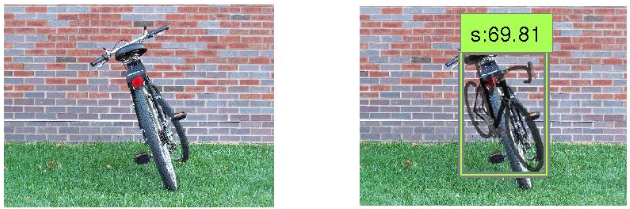
\includegraphics[width=0.40\linewidth]{supp/bicycle1.png} &
  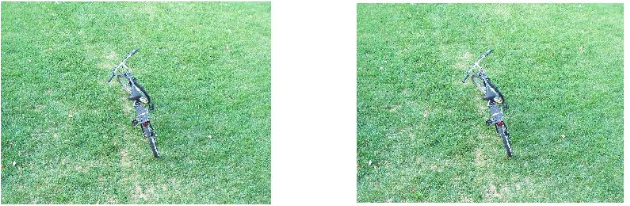
\includegraphics[width=0.40\linewidth]{supp/bicycle5.png} \\
  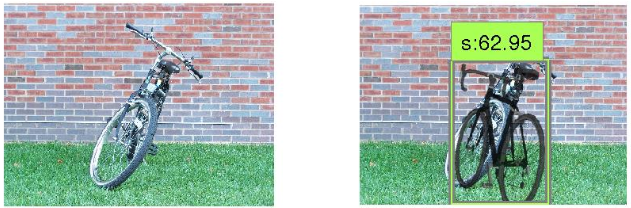
\includegraphics[width=0.40\linewidth]{supp/bicycle19.png} &
  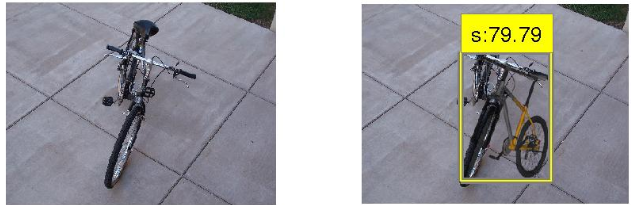
\includegraphics[width=0.40\linewidth]{supp/bicycle20.png} \\
\hline
\end{tabular}
\caption{Failed detection or pose estimation on 3D Object
  Classes~\cite{savarese07} bicycles. Original image (left) and overlaid
  detection result (right).}
  \label{fig:3dobject_bicycle_bad}
\end{figure*}

\section{Enriching Existing Detections}
%
It this section, we provide qualitative examples and plots for the experiment
``Enriching Existing Detections'' (Sect.~6.3 in the main paper).

To recapitulate, we enrich object detection bounding boxes from
a state-of-the-art detector (R-CNN~\cite{Girshick14}) with 2D-3D
registration and continuous viewpoint estimation. We present detection
average precision, average viewpoint precision, viewpoint confusion
matrix and mean precision in pose estimation results in
Fig.~\ref{fig:pascal_ap}, following the evaluation criteria
of~\cite{Xiang14} for detection and viewpoint
estimation. Fig.~\ref{fig:pascal3d_car_good} to
Fig.~\ref{fig:pascal3d_bicycle_bad} give qualitative results.
%
%In this experiment, we use R-CNN\cite{Girshick14} for detection bounding box
%proposals and our system produces accurate 2D-3D matching on the proposal
%regions.

We use $15\%$ context (extending the proposal region by $15\%$ on the
top, right, left, and bottom). We run our pipeline on the
PASCAL3D+~\cite{Xiang14} dataset, including our fine-tuning stage.
%
%If our method fails to estimate viewpoint (confidence score is below
%45), it
If our method fails to estimate viewpoint (confidence score is below a
threshold), it outputs 0 azimuth, 0 elevation, 0 yaw. Note that for
both categories and different numbers of viewpoints, our method has
difficulty distinguishing front and back views, but yields little
confusion between neighboring views. The failure cases given in
Fig.~\ref{fig:pascal3d_car_bad} and
Fig.~\ref{fig:pascal3d_bicycle_bad} are mostly caused by truncation,
occlusion, and unusual object shape.
%
\begin{figure*}[h]
  \centering
  \begin{tabular}{cc}
  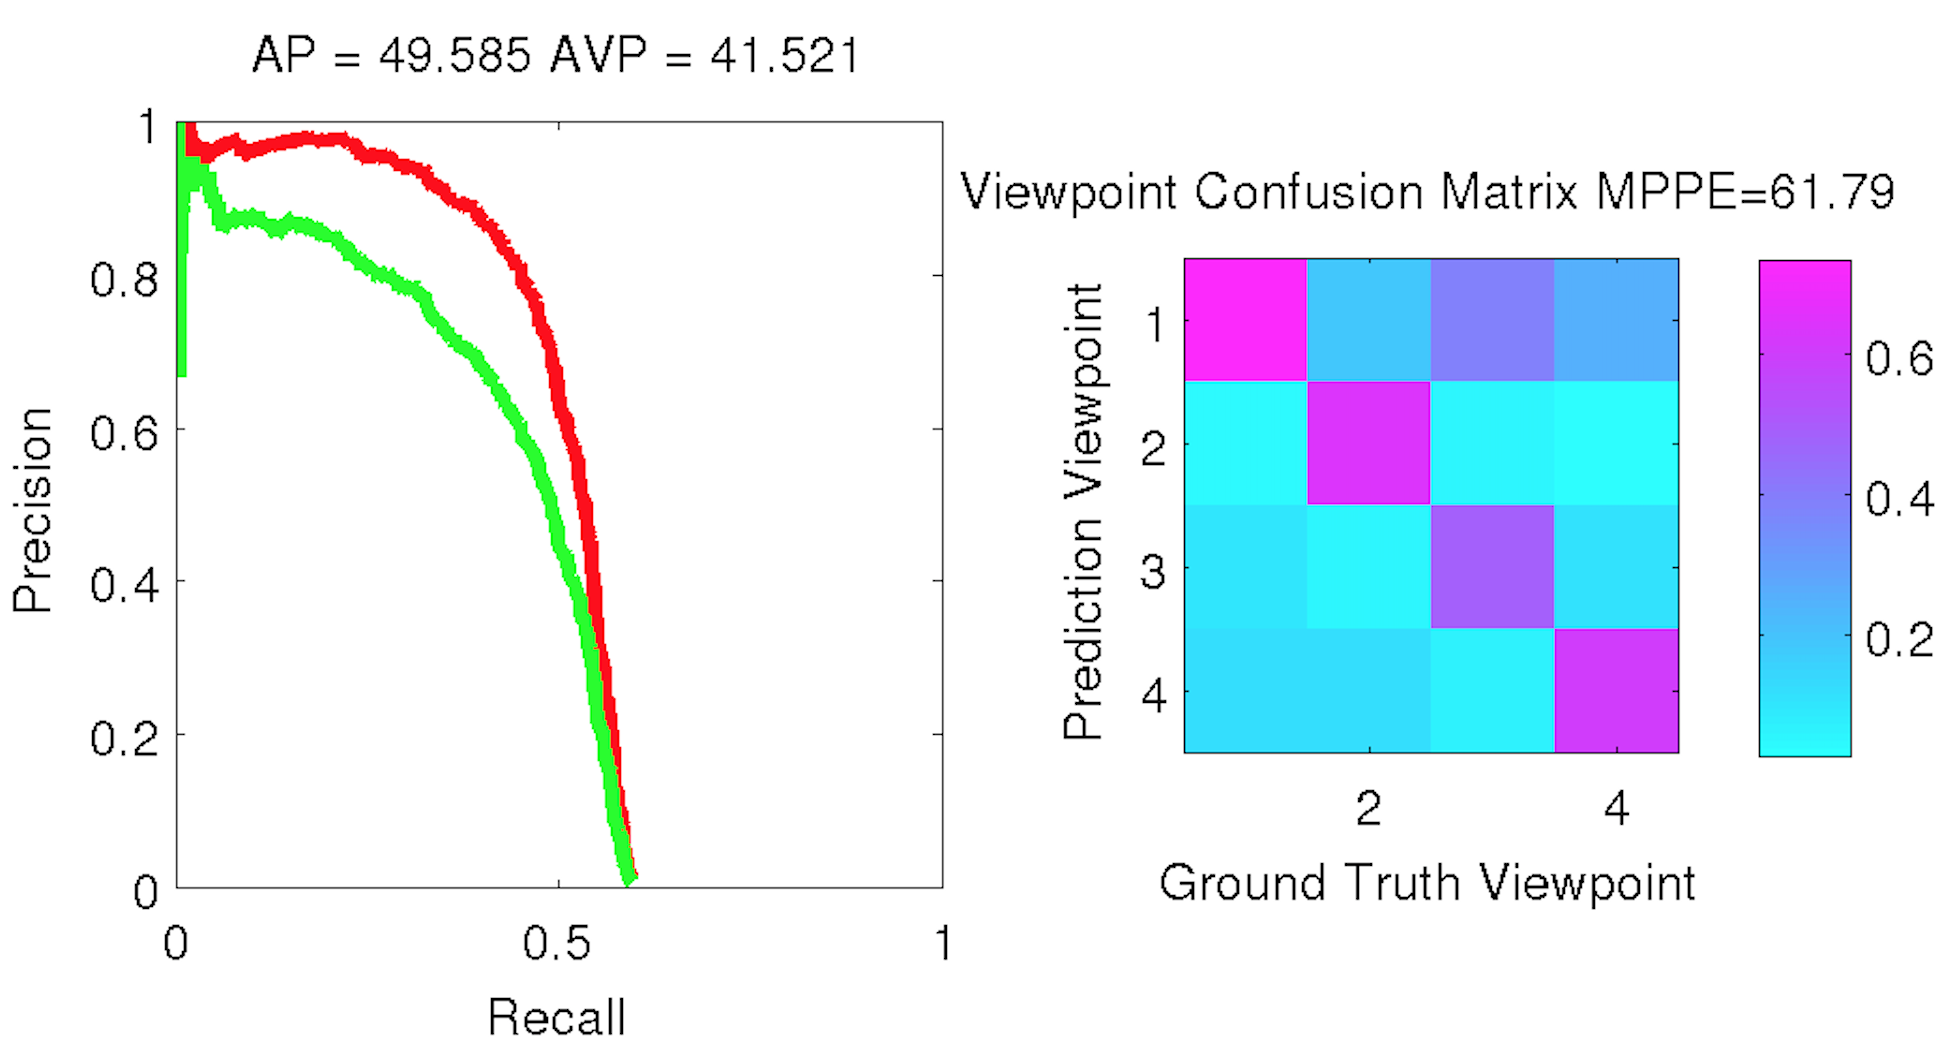
\includegraphics[width=0.45\linewidth]{car_cnn4_crop.png}&
  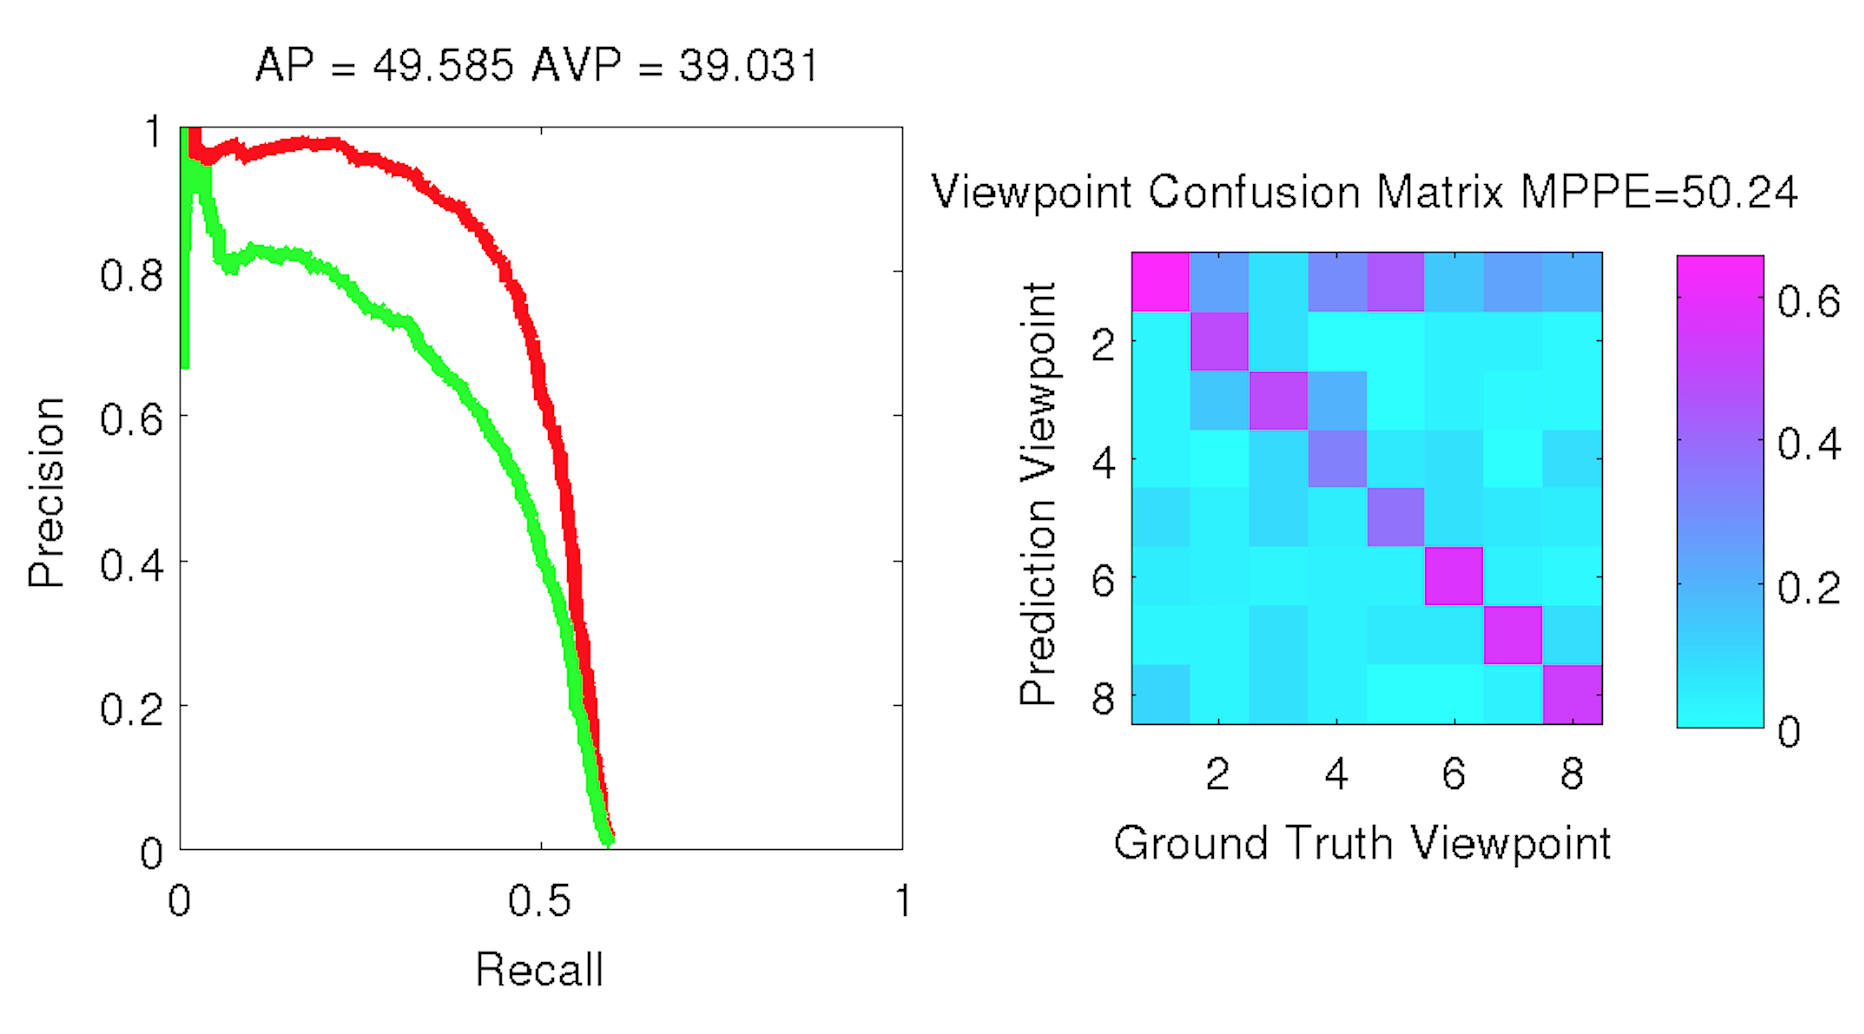
\includegraphics[width=0.45\linewidth]{car_cnn8_crop.png}\\
    (a) Car, 4 views&
    (b) Car, 8 views\\
  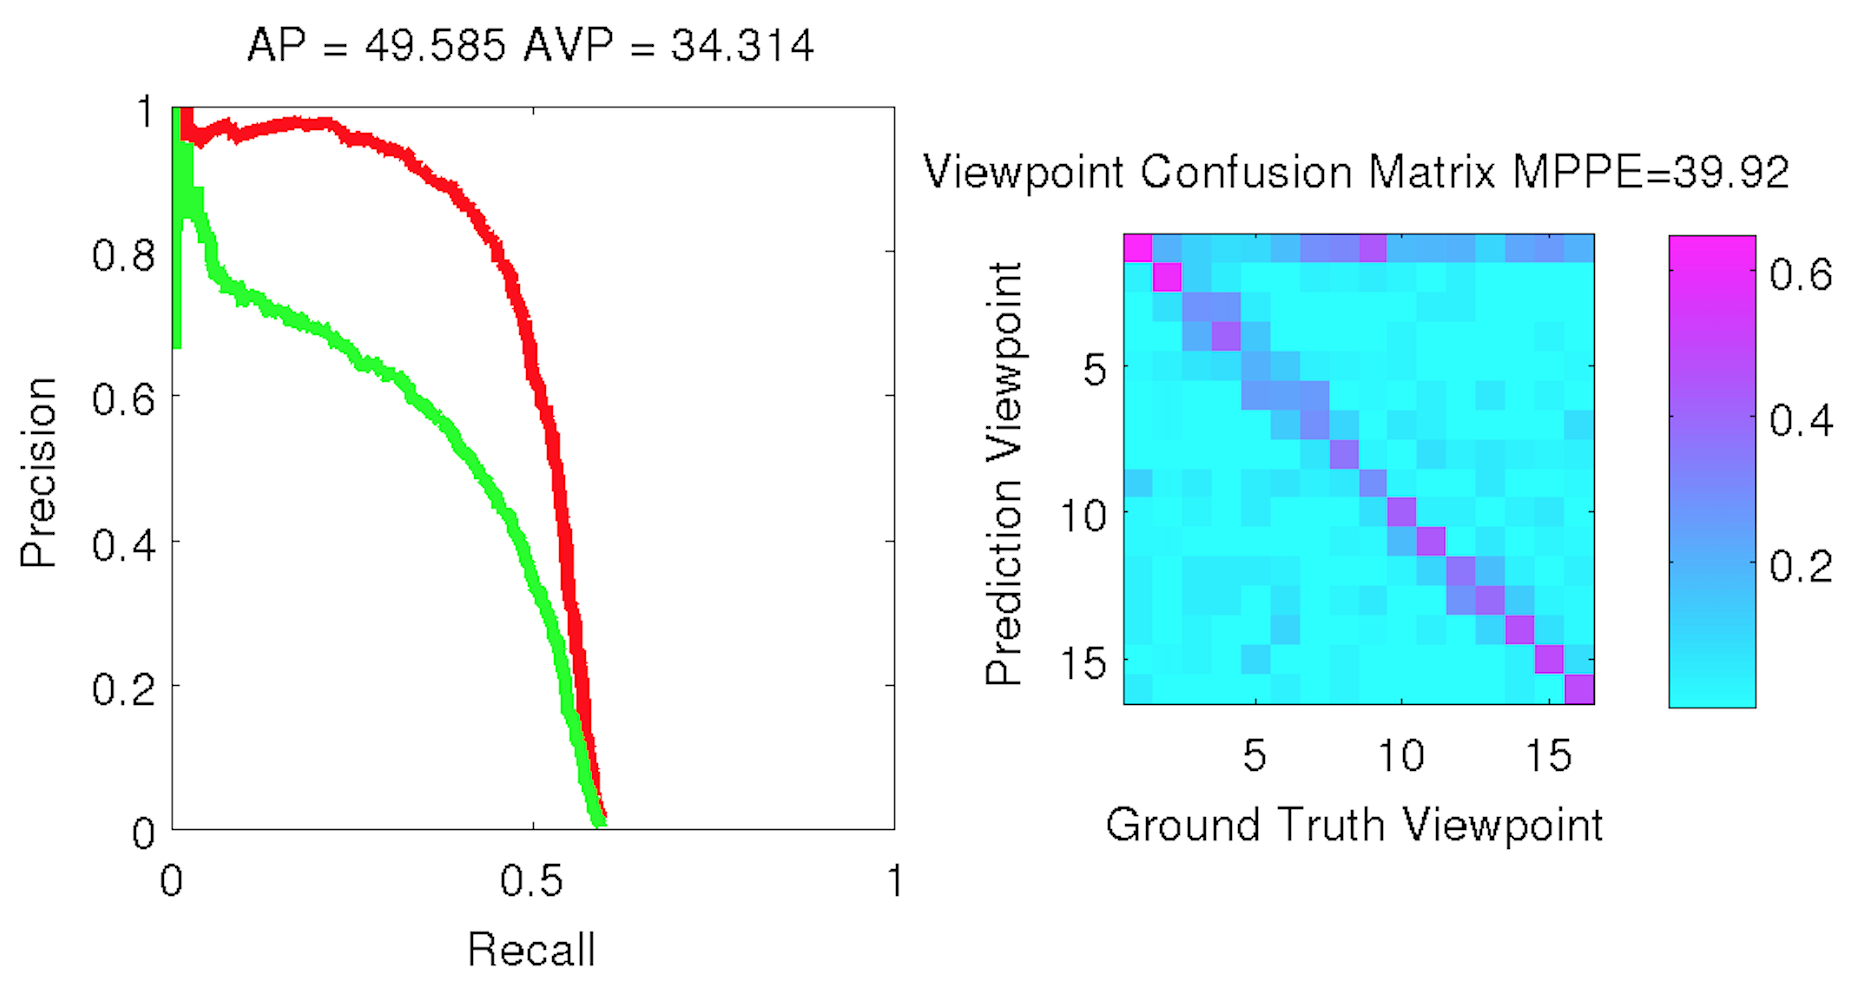
\includegraphics[width=0.45\linewidth]{car_cnn16_crop.png}&
  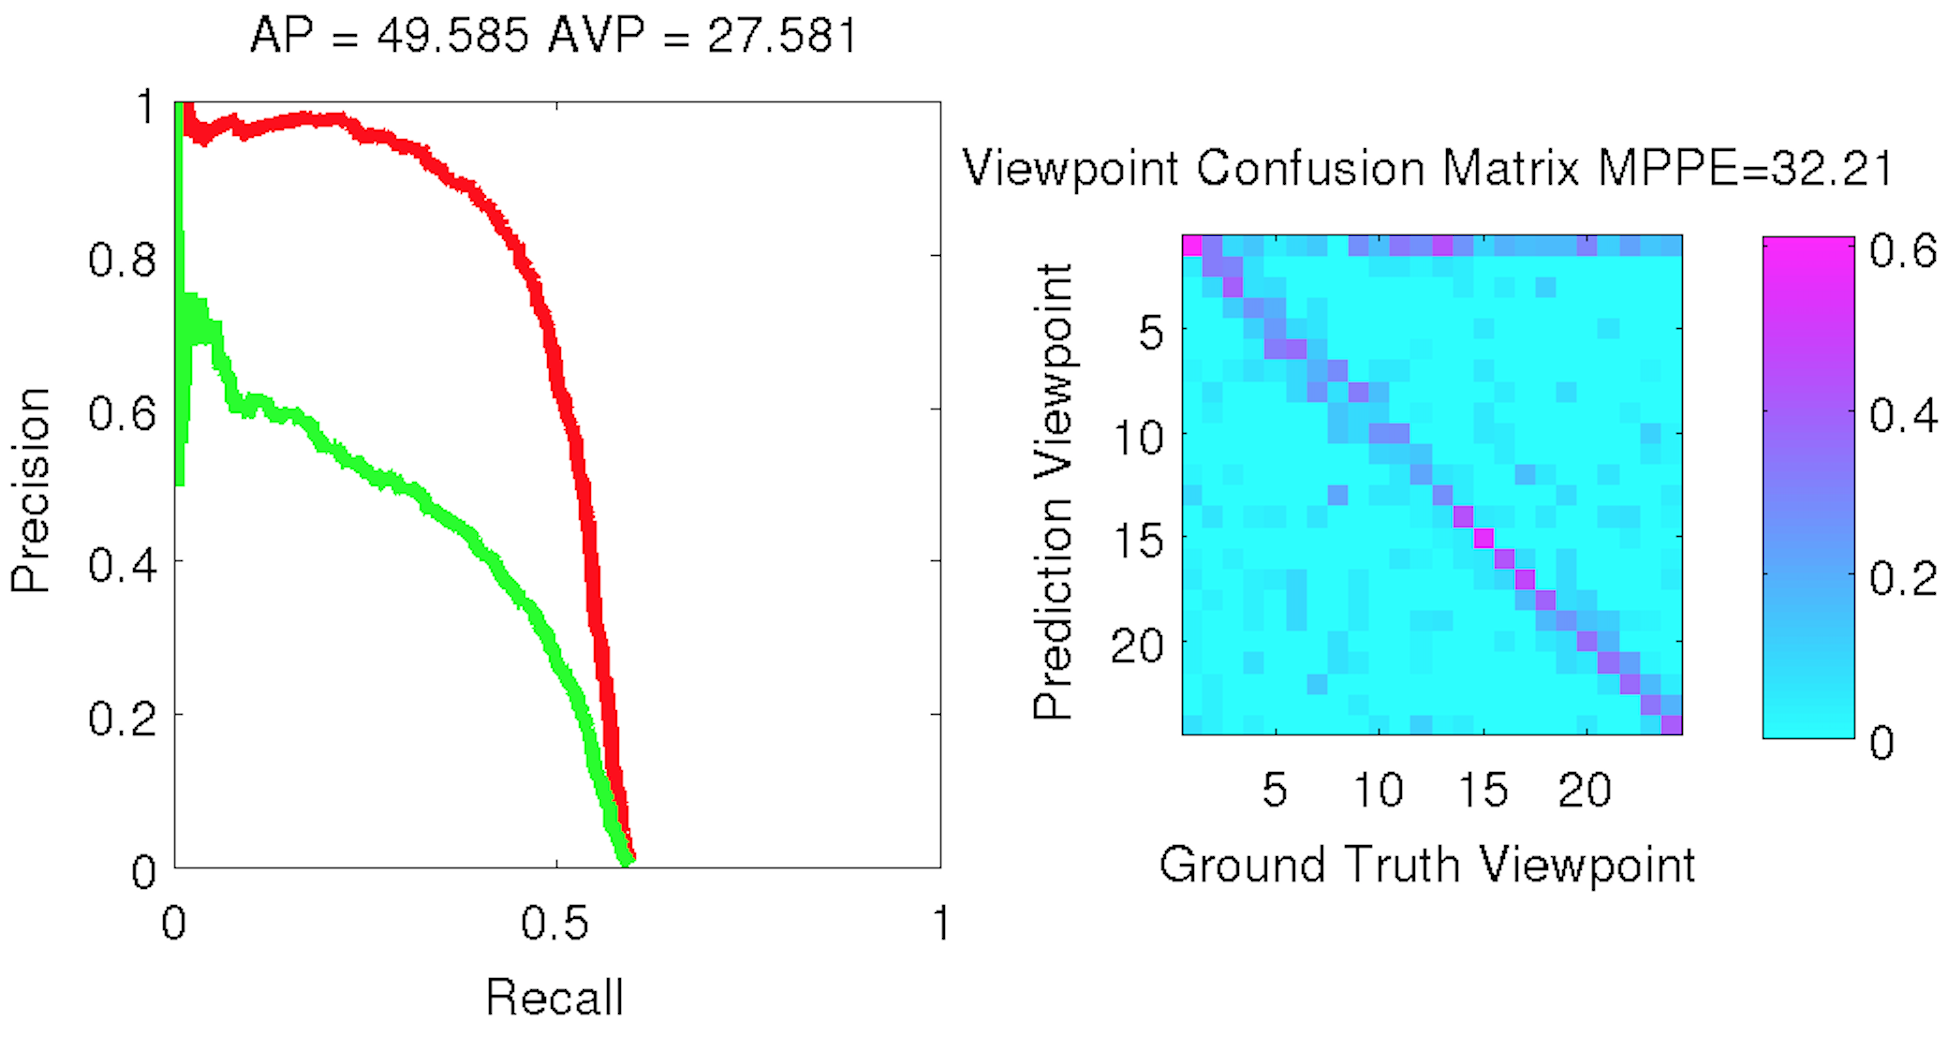
\includegraphics[width=0.45\linewidth]{car_cnn24_crop.png}\\
    (c) Car, 16 views&
    (d) Car, 24 views\\
  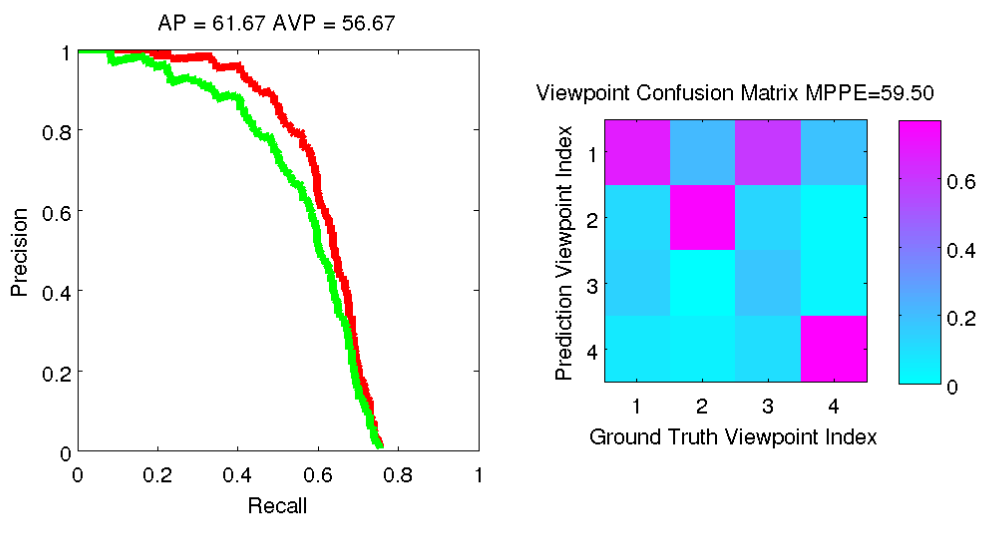
\includegraphics[width=0.45\linewidth]{supp/bicycle_cnn4_crop.png}&
  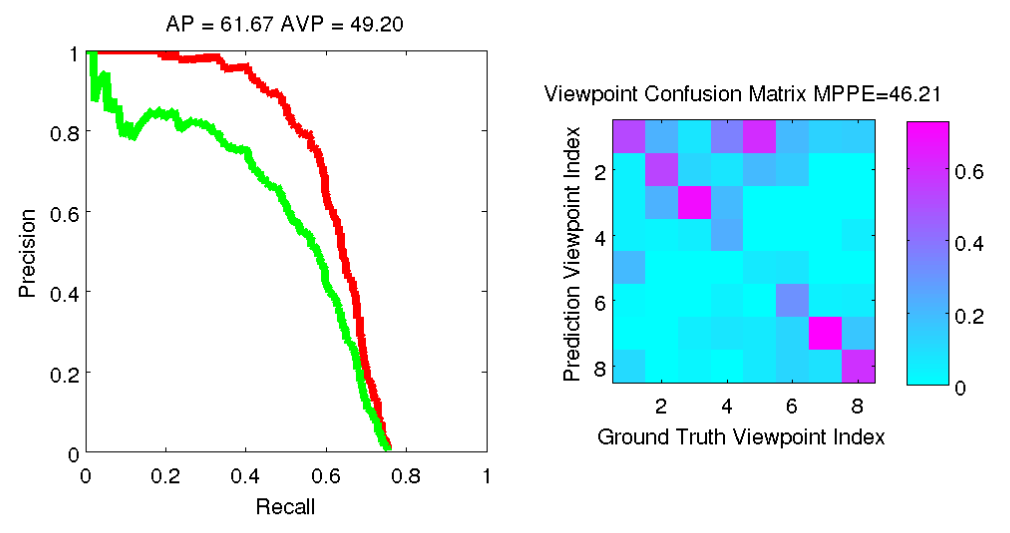
\includegraphics[width=0.45\linewidth]{supp/bicycle_cnn8_crop.png}\\
    (e) Bicycle, 4 views&
    (j) Bicycle, 8 views\\  
  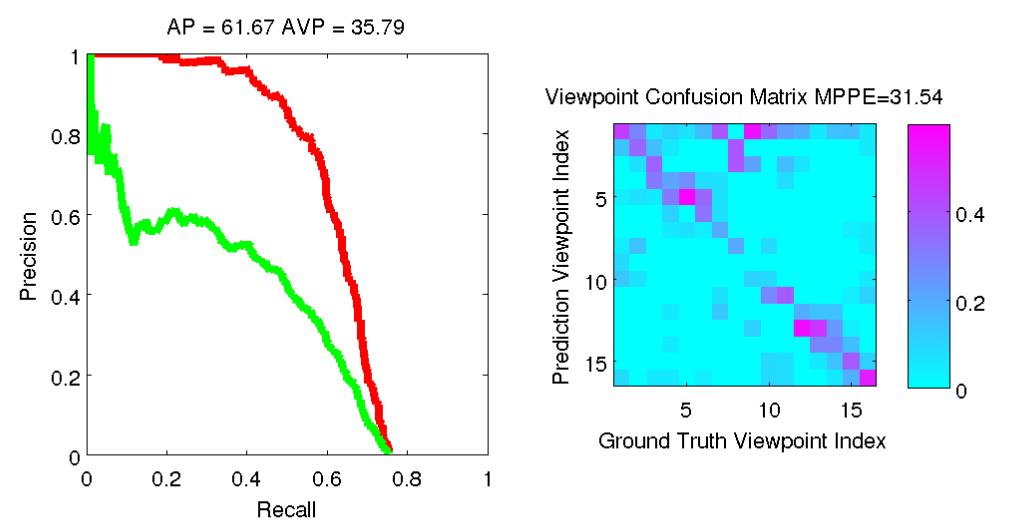
\includegraphics[width=0.45\linewidth]{supp/bicycle_cnn16_crop.png}&
  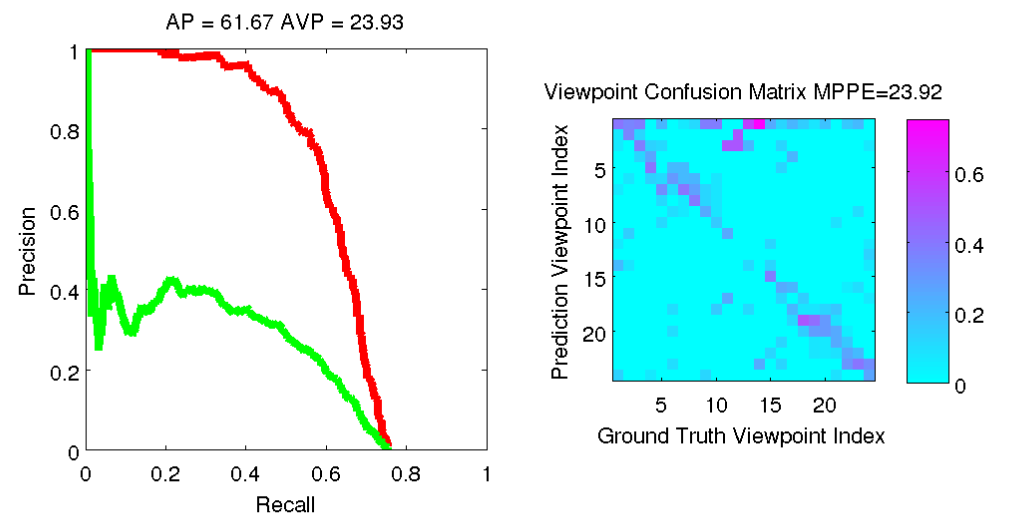
\includegraphics[width=0.45\linewidth]{supp/bicycle_cnn24_crop.png}\\
    (g) Bicycle, 16 views&
    (h) Bicycle, 24 views\\
  \end{tabular}
  \caption{Detection and pose estimation on PASCAL3D+~\cite{Xiang14}
    cars and bicycles.
    Average Precision (red) and Average Viewpoint Precision (green)
    are given in the left plot and viewpoint confusion table and MPPE
    are given in the right plot. The viewpoint index 1 is front, 2 is
    front-right, \dots, $n-1$ is front-left for number of viewpoints $n$.}
 % On the left, we
 %  present average precision curve (red) average viewpoint precision curve
 %  (green). On the right, we present confusion matrix and mean precision in pose
 %  estimation. Viewpoint index 1 is front, index 2 is front-right \dots and
 %  $n-1$ is front-left for number of viewpoints $n$.}
  \label{fig:pascal_ap}
\end{figure*}
%
\begin{figure*}[h]
\setlength\tabcolsep{1pt}
\centering
\begin{tabular}{|cc|cc|}
  \hline
  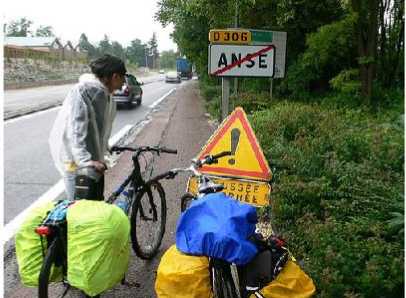
\includegraphics[width=0.24\linewidth]{supp/occlusion1.png} &
  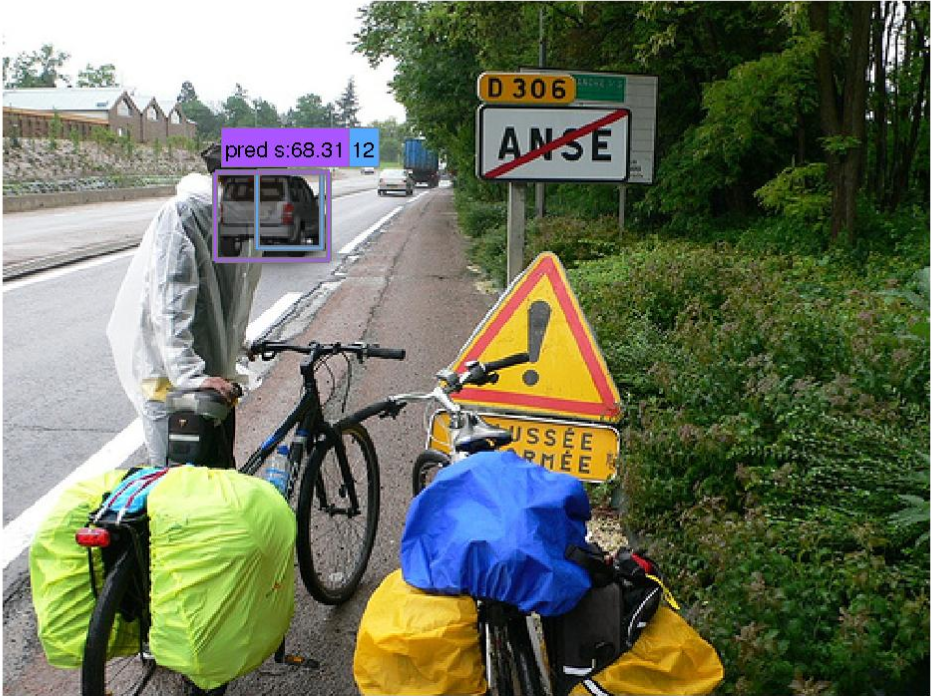
\includegraphics[width=0.24\linewidth]{supp/occlusion1b.png} & 
  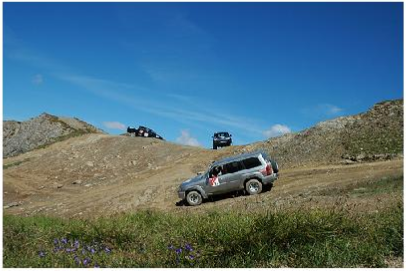
\includegraphics[width=0.24\linewidth]{supp/pas_car1a.png} &
  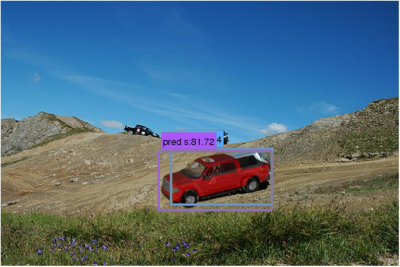
\includegraphics[width=0.24\linewidth]{supp/pas_car1b.png}  \\
  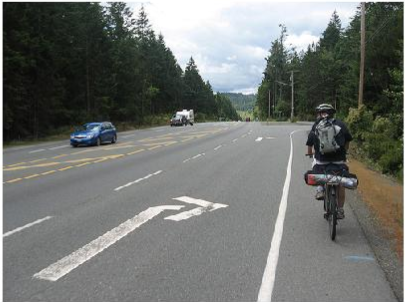
\includegraphics[width=0.24\linewidth]{supp/pas_car3a.png} &
  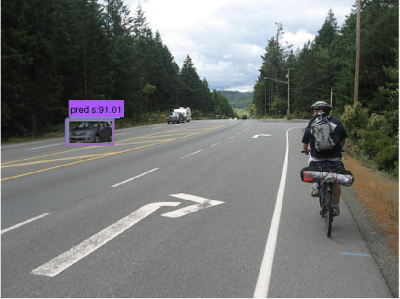
\includegraphics[width=0.24\linewidth]{supp/pas_car3b.png} & 
  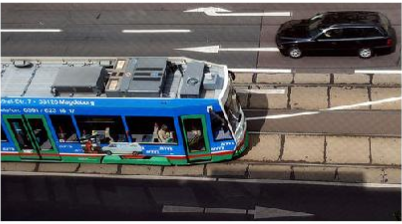
\includegraphics[width=0.24\linewidth]{supp/pas_car5a.png} &
  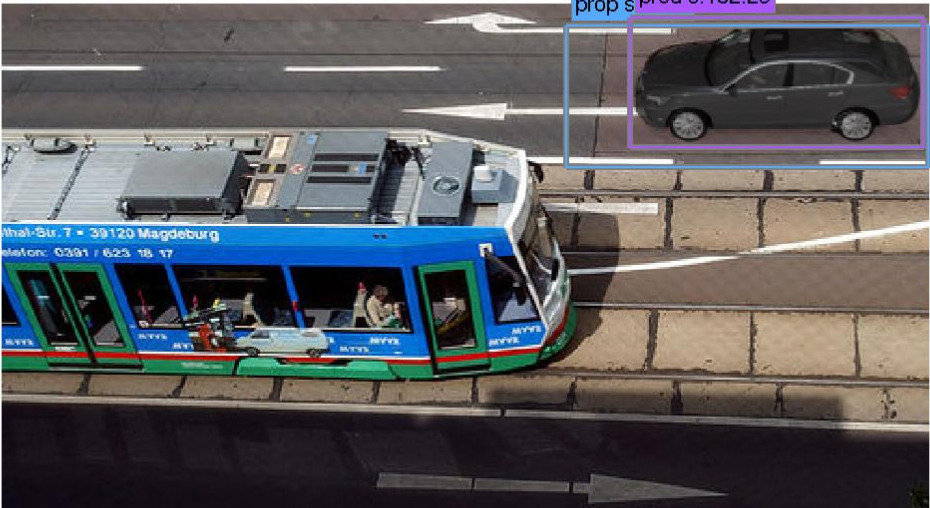
\includegraphics[width=0.24\linewidth]{supp/pas_car5b.png}  \\
  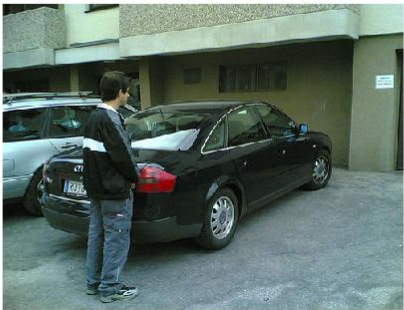
\includegraphics[width=0.24\linewidth]{supp/pas_car6a.png} &
  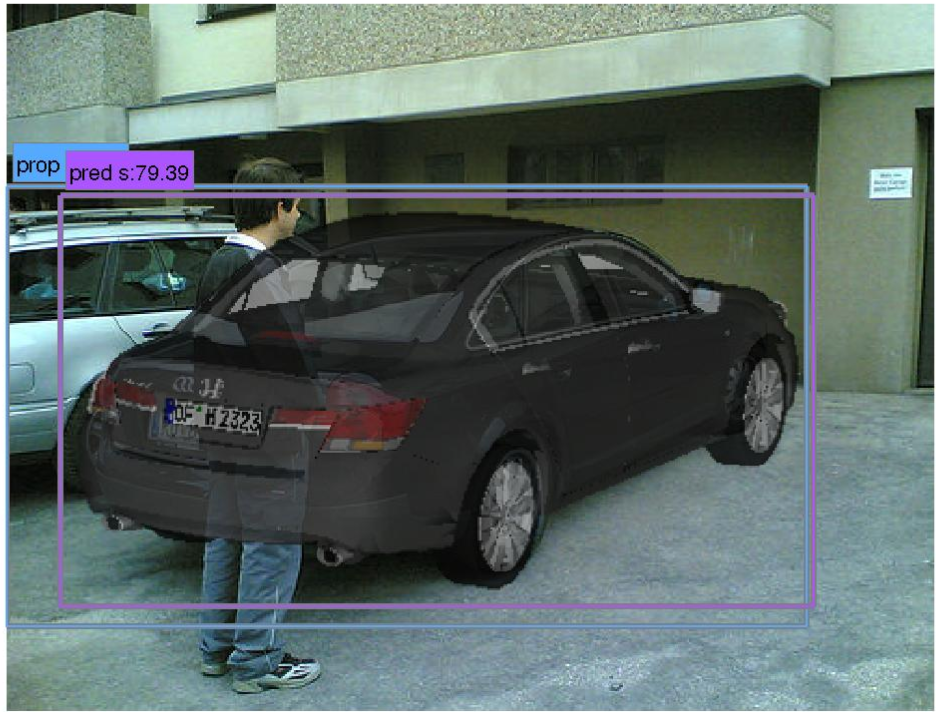
\includegraphics[width=0.24\linewidth]{supp/pas_car6b.png} & 
  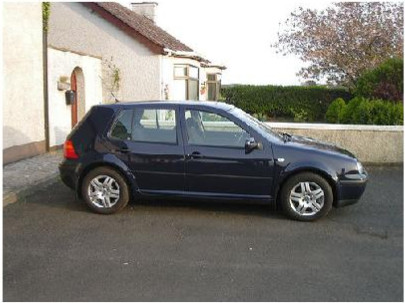
\includegraphics[width=0.24\linewidth]{supp/pas_car7a.png} &
  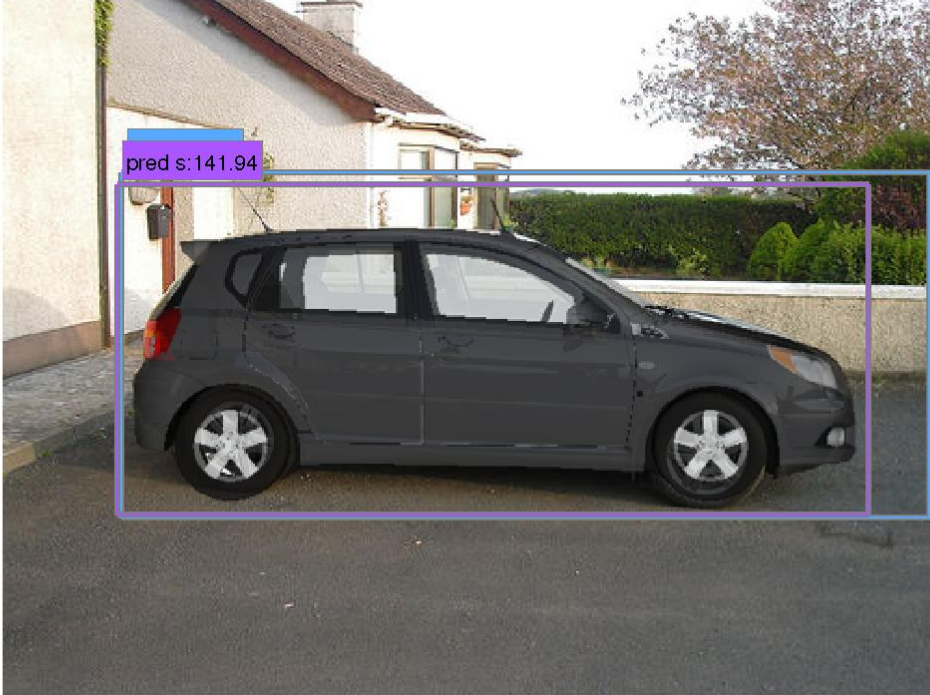
\includegraphics[width=0.24\linewidth]{supp/pas_car7b.png}  \\
  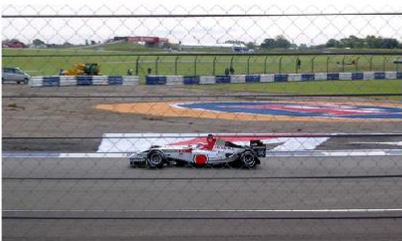
\includegraphics[width=0.24\linewidth]{supp/pas_car10a.png} &
  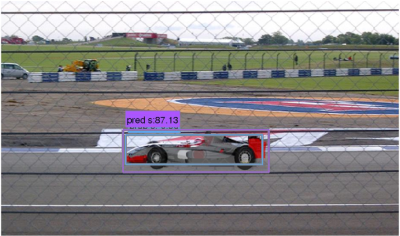
\includegraphics[width=0.24\linewidth]{supp/pas_car10b.png} & 
  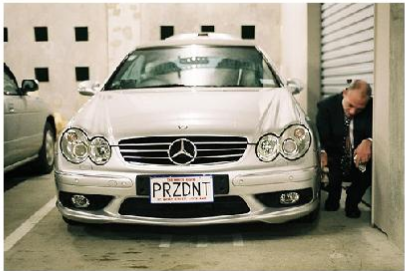
\includegraphics[width=0.24\linewidth]{supp/pas_car16a.png} &
  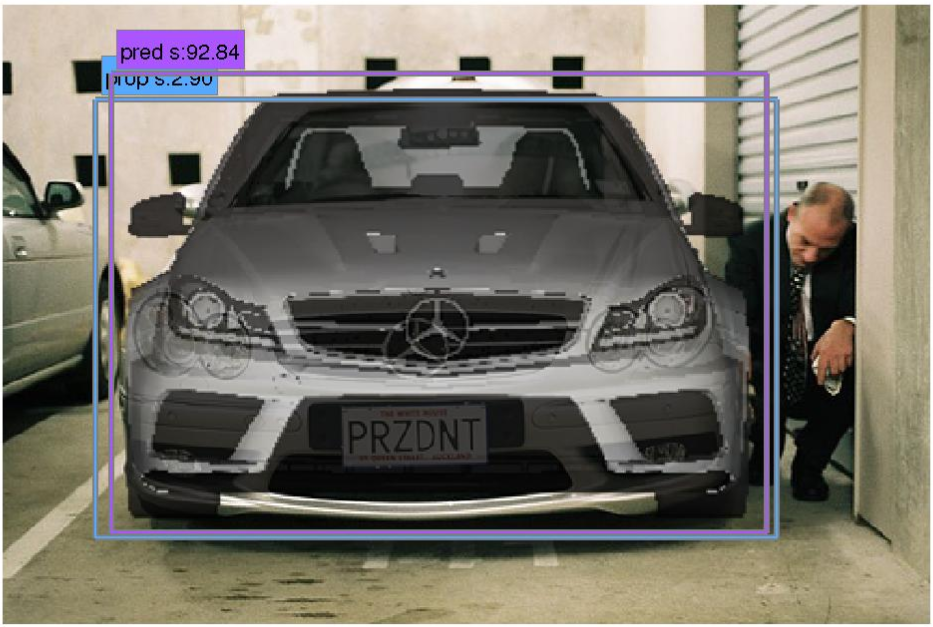
\includegraphics[width=0.24\linewidth]{supp/pas_car16b.png}  \\
  \includegraphics[width=0.24\linewidth]{supp/pas_car17a.png} &
  \includegraphics[width=0.24\linewidth]{supp/pas_car17b.png} & 
  \includegraphics[width=0.24\linewidth]{supp/pas_car19a.png} &
  \includegraphics[width=0.24\linewidth]{supp/pas_car19b.png} \\
  \includegraphics[width=0.24\linewidth]{supp/pas_car21a.png} &
  \includegraphics[width=0.24\linewidth]{supp/pas_car21b.png} & 
  \includegraphics[width=0.24\linewidth]{supp/pas_car22a.png} &
  \includegraphics[width=0.24\linewidth]{supp/pas_car22b.png} \\
  \includegraphics[width=0.24\linewidth]{supp/pas_car18a.png} &
  \includegraphics[width=0.24\linewidth]{supp/pas_car18b.png} & 
  \includegraphics[width=0.24\linewidth]{supp/pas_car18c.png} &
  \includegraphics[width=0.24\linewidth]{supp/pas_car18d.png} \\
  \hline
  \end{tabular}
  \caption{Successful detection and pose estimation result on PASCAL3D+ dataset
  car category, On each column, original image is on the left and overlaid
  2D-3D registration on the right with a proposal bounding box (blue) and a
  predicted bounding box (purple).} 
  \label{fig:pascal3d_car_good}
\end{figure*}


\begin{figure*}[h]
\setlength\tabcolsep{1pt}
\centering
\begin{tabular}{|cc|cc|}
  \hline
  \includegraphics[width=0.22\linewidth]{supp/pas_bicycle3a.png} &
  \includegraphics[width=0.22\linewidth]{supp/pas_bicycle3b.png} & 
  \includegraphics[width=0.22\linewidth]{supp/pas_bicycle13a.png} &
  \includegraphics[width=0.22\linewidth]{supp/pas_bicycle13b.png}  \\
  \includegraphics[width=0.22\linewidth]{supp/pas_bicycle5a.png} &
  \includegraphics[width=0.22\linewidth]{supp/pas_bicycle5b.png} & 
  \includegraphics[width=0.22\linewidth]{supp/pas_bicycle6a.png} &
  \includegraphics[width=0.22\linewidth]{supp/pas_bicycle6b.png}  \\
  \includegraphics[width=0.15\linewidth]{supp/pas_bicycle7a.png} &
  \includegraphics[width=0.15\linewidth]{supp/pas_bicycle7b.png} & 
  \includegraphics[width=0.22\linewidth]{supp/pas_bicycle8a.png} &
  \includegraphics[width=0.22\linewidth]{supp/pas_bicycle8b.png}  \\
  \includegraphics[width=0.15\linewidth]{supp/pas_bicycle9a.png} &
  \includegraphics[width=0.15\linewidth]{supp/pas_bicycle9b.png} & 
  \includegraphics[width=0.22\linewidth]{supp/pas_bicycle10a.png} &
  \includegraphics[width=0.22\linewidth]{supp/pas_bicycle10b.png}  \\
  \includegraphics[width=0.22\linewidth]{supp/pas_bicycle1a.png} &
  \includegraphics[width=0.22\linewidth]{supp/pas_bicycle1b.png} & 
  \includegraphics[width=0.22\linewidth]{supp/pas_bicycle2a.png} &
  \includegraphics[width=0.22\linewidth]{supp/pas_bicycle2b.png}  \\
  \includegraphics[width=0.22\linewidth]{supp/pas_bicycle11a.png} &
  \includegraphics[width=0.22\linewidth]{supp/pas_bicycle11b.png} & 
  \includegraphics[width=0.22\linewidth]{supp/pas_bicycle12a.png} &
  \includegraphics[width=0.22\linewidth]{supp/pas_bicycle12b.png}  \\
  \hline
  \end{tabular}
\caption{Successful detection and pose estimation result on PASCAL3D+ dataset
  bicycle category, On each column, original image is on the left and overlaid
  2D-3D registration on the right with a proposal bounding box (blue) and a
  predicted bounding box (purple).} 
  \label{fig:pascal3d_bicycle_good}
\end{figure*}


\begin{figure*}[h]
\setlength\tabcolsep{1pt}
\centering
\begin{tabular}{|cc|cc|}
  \hline
%   \includegraphics[width=0.24\linewidth]{supp/pas_car2a.png} &
%   \includegraphics[width=0.24\linewidth]{supp/pas_car2b.png} & 
%   \includegraphics[width=0.24\linewidth]{supp/pas_car4a.png} &
%   \includegraphics[width=0.24\linewidth]{supp/pas_car4b.png} \\
  \includegraphics[width=0.22\linewidth]{supp/pas_car8a.png} &
  \includegraphics[width=0.22\linewidth]{supp/pas_car8b.png} & 
  \includegraphics[width=0.22\linewidth]{supp/pas_car9a.png} &
  \includegraphics[width=0.22\linewidth]{supp/pas_car9b.png} \\ 
  \includegraphics[width=0.22\linewidth]{supp/pas_car11a.png} &
  \includegraphics[width=0.22\linewidth]{supp/pas_car11b.png} & 
  \includegraphics[width=0.22\linewidth]{supp/pas_car12a.png} &
  \includegraphics[width=0.22\linewidth]{supp/pas_car12b.png} \\
  \includegraphics[width=0.22\linewidth]{supp/pas_car14a.png} &
  \includegraphics[width=0.22\linewidth]{supp/pas_car14b.png} & 
  \includegraphics[width=0.22\linewidth]{supp/pas_car15a.png} &
  \includegraphics[width=0.22\linewidth]{supp/pas_car15.png} \\ 
  \includegraphics[width=0.22\linewidth]{supp/pas_car20a.png} &
  \includegraphics[width=0.22\linewidth]{supp/pas_car20b.png} &
  \includegraphics[width=0.22\linewidth]{supp/pas_car23a.png} &
  \includegraphics[width=0.22\linewidth]{supp/pas_car23b.png} \\
  \hline
  \end{tabular}
\caption{Failed detection or pose estimation result on PASCAL3D+ dataset
  car category, On each column, original image is on the left and overlaid
  2D-3D registration on the right with a proposal bounding box (blue) and a
  predicted bounding box (purple).} 
  \label{fig:pascal3d_car_bad}
\end{figure*}


\begin{figure*}[h]
\setlength\tabcolsep{1pt}
\centering
\begin{tabular}{|cc|cc|}
  \hline
  \includegraphics[width=0.22\linewidth]{supp/pas_bicycle14a.png} &
  \includegraphics[width=0.22\linewidth]{supp/pas_bicycle14b.png} & 
  \includegraphics[width=0.15\linewidth]{supp/pas_bicycle15a.png}  &
  \includegraphics[width=0.15\linewidth]{supp/pas_bicycle15b.png}  \\
  \includegraphics[width=0.22\linewidth]{supp/pas_bicycle16a.png} &
  \includegraphics[width=0.22\linewidth]{supp/pas_bicycle16b.png} & 
  \includegraphics[width=0.22\linewidth]{supp/pas_bicycle17a.png}  &
  \includegraphics[width=0.22\linewidth]{supp/pas_bicycle17b.png}  \\ 
  \includegraphics[width=0.22\linewidth]{supp/pas_bicycle18a.png} &
  \includegraphics[width=0.22\linewidth]{supp/pas_bicycle18b.png} & 
  \includegraphics[width=0.22\linewidth]{supp/pas_bicycle19a.png}  &
  \includegraphics[width=0.22\linewidth]{supp/pas_bicycle19b.png}  \\   \hline
  \end{tabular}
\caption{Failed detection or pose estimation result on PASCAL3D+ dataset
  bicycle category, On each column, original image is on the left and overlaid
  2D-3D registration on the right with a proposal bounding box (blue) and a
  predicted bounding box (purple).} 
  \label{fig:pascal3d_bicycle_bad}
\end{figure*}


\section{Fine Tuning}
Lastly, we provide qualitative examples of the fine-tuning stage of
our pipeline based on MCMC sampling (Sect.~5 in the main paper) in
Fig.~\ref{fig:tuning}. Please note that, while the visual difference
appear subtle, our method often manages to improve upon the initial
pose estimate.
%
\begin{figure*}[h]
\setlength\tabcolsep{1pt}
\centering
\begin{tabular}{ccc}
  \includegraphics[width=0.22\linewidth]{supp/tuning_1a.png} &
  \includegraphics[width=0.22\linewidth]{supp/tuning_1b.png} & 
  \includegraphics[width=0.22\linewidth]{supp/tuning_1c.png}  \\
  \includegraphics[width=0.22\linewidth]{supp/tuning_2a.png} &
  \includegraphics[width=0.22\linewidth]{supp/tuning_2b.png} & 
  \includegraphics[width=0.22\linewidth]{supp/tuning_2c.png}  \\ 
  \includegraphics[width=0.22\linewidth]{supp/tuning_3a.png} &
  \includegraphics[width=0.22\linewidth]{supp/tuning_3b.png} & 
  \includegraphics[width=0.22\linewidth]{supp/tuning_3c.png}  \\   
  \includegraphics[width=0.22\linewidth]{supp/tuning_4a.png} &
  \includegraphics[width=0.22\linewidth]{supp/tuning_4b.png} & 
  \includegraphics[width=0.22\linewidth]{supp/tuning_4c.png}  \\     
  \includegraphics[width=0.22\linewidth]{supp/tuning_5a.png} &
  \includegraphics[width=0.22\linewidth]{supp/tuning_5b.png} & 
  \includegraphics[width=0.22\linewidth]{supp/tuning_5c.png}  \\
  \includegraphics[width=0.22\linewidth]{supp/tuning_6a.png} &
  \includegraphics[width=0.22\linewidth]{supp/tuning_6b.png} & 
  \includegraphics[width=0.22\linewidth]{supp/tuning_6c.png}  \\
  \end{tabular}
\caption{From left to right, original images, initial pose estimations and
fine-tuned result. The numbers, from the left, indicate detection confidence
and intersection over union respectively.} 
  \label{fig:tuning}
\end{figure*}


{\small
\bibliographystyle{ieee}
\bibliography{egbib}
}

\end{document}
